
%% add noise image
\begin{figure}[!h]
	\centering
	\begin{tikzpicture}
		\node[inner sep=0pt] (depthmap) at (0,0)
		{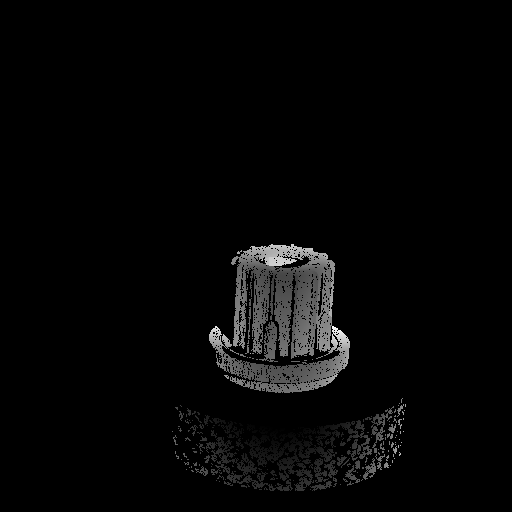
\includegraphics[width=.6\textwidth]{./pic/00028.depth0.png}};
	\end{tikzpicture}
	\caption{A depth map captured via infrared sensors. The dark pixels close to the camera, the light pixels away to the camera. The missing pixels distributed all of the image.}
	\label{fig:depth_map_with_noise}
\end{figure}


%% add noise image
\begin{figure}[!h]
	\centering
	\begin{tikzpicture}	
		\node[inner sep=0pt] (normal) at (8,0)
		{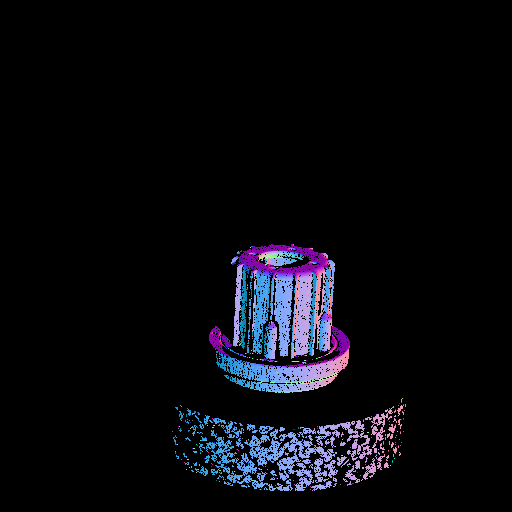
\includegraphics[width=.6\textwidth]{./pic/00028.normal0.png}};
	\end{tikzpicture}
	\caption{Semi-dense Normal Map calculated from depth map using standard method}
	\label{fig:standard_normal_inference}
\end{figure}





%%%%%%%%%%%%%%%%%%%%%%%%%%%%%%%%%%%%%%%%%%%%%% intro %%%%%%%%%%%%%%%%%%%%%%%%%%%%%%%%%%%%%%%%%%%%%% 

%% What is surface normal
\section{Introduction}
In three dimension geometry, a surface normal at the point $ P $ is a vector $ n $ perpendicular to the tangent plane of the surface at point $ P $. The length of a normal is usually one, with a sign to represent the sides (interior or exterior).


%% why surface normal is important
Surface normal has many practical applications, such as augmented reality and robotics. In these applications, normal impacts on the way that objects are represented. Some tasks such as surface reconstruction, image registration, shading, etc, they all required surface normal as one of the inputs. 


%%%%%%%%%%%%%%%%%%% talk about the reason of this thesis %%%%%%%%%%%%%%%%%%

%% standard method for normal inference is insufficient, input is sparse, not robust enough
Standard methods compute normals from point cloud using neighboring information in image space or from a single grayscale image using use Shape from Shading \cite{SFS}. The first method bases on the assumption that the neighbors of the points are located on the same plane. It performs well with a well-chosen window size. The drawbacks are, the algorithm is highly noise sensitive. It is weak with handling missing pixels, which is a common issue in the input data. The second method depends on the correct information about light source. Errors may occur in regions with inter-reflections in the 3D measurement. 

%% CNN based methods
Recently, deep learning based method \cite{yolov3}, \cite{efficientDet} achieved a great succeed for image processing. 
These kinds of network architecture takes a batch of RGB/Grayscale images as input which usually employed for classification problems. The image is usually convoluted with convolutional layer and downsampling with pooling layers. The outputs of the network consists of a single value to represent the index of corresponding class \cite{efficientDet}, or with set of values to represent the position of bounding boxes.\cite{yolov3}. 

%%%%%%%%%%%%%%%%%%% talk about the chanllege of this task %%%%%%%%%%%%%%%%%%
%% talk about the reason we need new type of network architecture
However, in many other vision tasks, like normal map inference, the output is demanded that it has the same shape as the input. Instead of predicting one or several classes for the whole input matrix, the classes for each pixels are required for prediction. In this case, the traditional network architecture is not suitable anymore.

%% talk about upsampling 
Recently, deep learning based methods are also applied on some computer vision tasks such as image segmentation, image inpainting and depth density enhancement. In these methods, multiple architectures have been proposed with an upsampling section. In this case, the output can be designed has the same shape as input or slightly smaller. Nevertheless, the resolution is similar to the input image. Normal Inference task has similar pipeline comparing to these tasks.

%% there exists space for improvment 
On the other hand, the point clouds data provided by Kinect or similar RGB-D, LiDAR sensors are only semi-dense. A huge mount of missing pixels distribute all over the images, some of the regions leave complete empty holes. This situation imposes another challenge on the normal inference. 

The depth image is incomplete, however, the depth sensor usually able to capture grayscale texture image, which are typically fully dense due to their passive nature. Furthermore, if the texture image is already illuminated by strong directional light of a video projector, whose position is known, then there should exist theoretical relations between light direction, normal direction, and grayscale image . Thus the normal can be inferenced better using the given image information and depth map.  Based grayscale image and corresponding semi-dense depth map, a CNN model can be designed to inference the normal map, which is able to give more density and robust result comparing to standard algorithm. 




%%%%%%%%%%%%%%%%%% talk about the main work in this thesis  %%%%%%%%%%%%%%%%%%
In this thesis, we found a solution for the problems mentioned above and proposed a noval deep learning architecture for surface normal inference.A network named Albedo Gated Normal Inference Network(AlGaN) is proposed to infer normal given the corresponding depth map. The architecture of AlGaN involves a two-stage CNN. The first stage infers the normal map using point cloud as input. If the light source position and grayscale image can be provided further, the second stage infers the albedo altogether with the normals from first stage. In addition, the loss function is based on least-square-error and Lambertian reflection.

With the help of synthetic data in Unity, a dataset is created for CNN model training. It can provide accurate ground-truth for training work, which real data usually not provided. The results on this dataset shows that our AlGaN model performs also well on real data captured by Infrared cameras. The trained Normal models achieve a remarkably better prediction accuracy at a low computational cost comparing to the standard approaches for semi-dense point clouds. 





